%IV - Algorithmes transformers - presolveurs - solveurs
%    1. Transformers
%    1.1 Simple Transformer[dodo]
%    1.2 Hole Transformer[elodie]
%    
%    2. Solveurs et leur presolveurs
%    2.1 ToInfinityAndBeyond
%    2.2 TheSkyIsTheLimit
%    2.3 ScanLine
%    (2.4 Solveur physique)
%    (2.5 Solveur probabiliste)


%% Rappel : à ce moment du rapport, on a déjà expliqué l'architecture du code - PLEASE DO NOT REPEAT ;)

%% TRANSFORMERS
\subsection{Transformers}
La classe Transformer a pour but de regrouper plusieurs sous-ensembles de formes en 'blocs'. Ce sont des algorithmes appliqués sur les formes avant l'étape de packing, ils servent à augmenter l'efficacité globale du programme, en cherchant des formes à assembler ensemble selon différents critères : les formes d'un 'bloc' sont choisies de manière à ce que l'aire occupée par le bloc soit la plus faible possible.
Certains transformers utilisent plusieurs critères de qualité : aire d'intersection entre enveloppes convexes, taille de la bounding box résultante etc.

L'intérêt de la classe Transformer est de pouvoir proposer un packing plus optimal qu'un algorithme solveur, mais seulement de manière locale (temps d'exécution qualitativement excessif).

En fin de tâche, la classe Transformer envoie un ensemble d'informations à la classe Merger pour que celle-ci puisse modifier la représentation interne des formes afin que les algorithmes suivants considèrent effectivement les formes déplacées comme un bloc insécable.


\subsubsection{Simple Transformer}

\indent Le \texttt{Simple Transformer} est un algorithme de packing \textit{brute force} qui, pour deux formes données, teste un ensemble de dispositions entre elles pour optimiser un critère de l'union résultante.\\

Pour cela, on effectue une série de rotations de la première forme sur elle-même, d'un angle $\alpha$. Puis on effectue une autre série de rotations d'un angle $\beta$ sur la seconde forme de la même façon. Pour chaque couple de rotations, la seconde forme est ensuite déplacée de façon à être alignée avec la première forme, selon l'axe $x$. Un léger \textit{offset} selon l'axe $y$ est ajouté pour tester toutes les configurations possibles (à la précision de l'\textit{offset} et des angles près). 

On minimise la distance entre les deux formes en translatant la deuxième selon l'axe des $x$, jusqu'à ce que les deux pièces se touchent, le tout par dichotomie. Tout le procédé est illustré en figure~\ref{fig:simpletransformer}.\\

On garde finalement le triplet $(\alpha, \beta, offset)$ minimisant un certain critère, passé en paramètre. Nous avons par exemple la minimisation de la bounding box résultante (utile lorsqu'on va utiliser un algorithme sur rectangles ensuite) ou bien la maximisation de l'aire d'intersection entre les enveloppes convexes.


\begin{figure}[!htb]
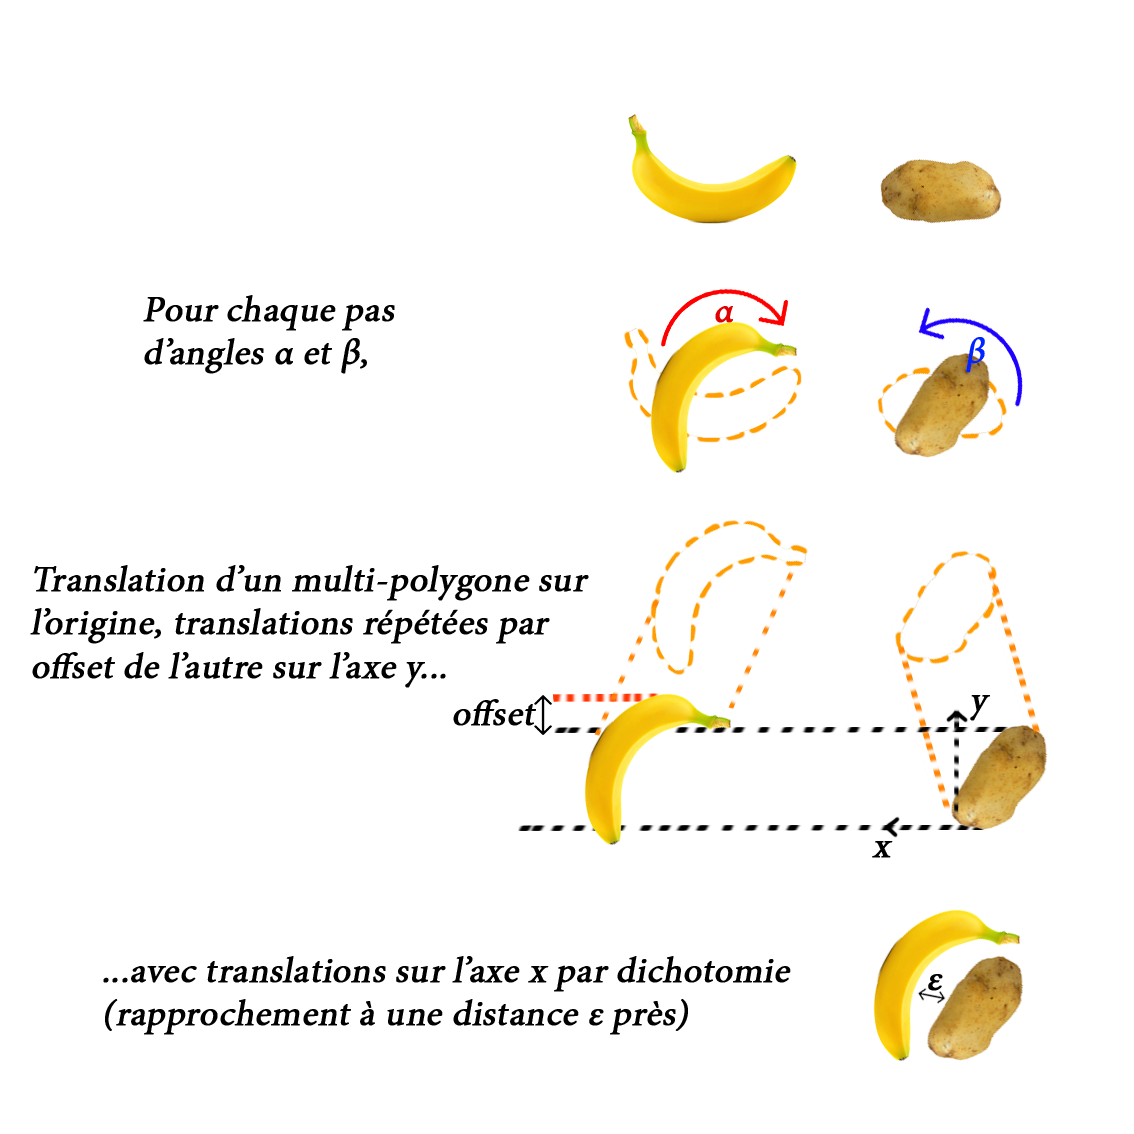
\includegraphics[scale=0.4]{img/simpletransformer.png}
\caption{Illustration du procédé de \texttt{SimpleTransformer}}
\label{fig:simpletransformer}
\end{figure}
%banana for scale

\subsubsection{Hole Transformer}
Le but de cet algorithme est de remplir les trous de formes trouées avec d'autres pièces de l'ensemble de Shapes. Cette étape peut s'avérer utile car dans les solveurs employés par la suite, on utilise au mieux les enveloppes extérieures des formes, sinon leur bounding box, empêchant ainsi toute pièce de jamais combler les trous d'une autre. 

Le pseudo-algorithme \ref{alg:hole} ci-dessous décrit le fonctionnement de ce transformer.

\begin{algorithm}
    \caption{- Hole Transformer}
    \label{alg:hole}   
    \textbf{Entrée} : Ensemble de formes\\
    \textbf{Sortie} : Vecteur de n-uplets des indices de formes à fusionner, avec leur nouvelle position\\

    \textbf{Début}\\
    \hspace{0.5cm}Établir une liste des trous triés par ordre décroissant d'aire;\\
    \hspace{0.5cm}Trier les formes par ordre croissant d'aire;\\
    \hspace{0.5cm}\textbf{Pour chaque} trou t :\\
        \hspace{1cm}\textbf{Pour chaque} forme f :\\
        \hspace{1cm}\textbf{Si} aire(f) < aire(t) \textbf{et} f n'a pas déjà été choisie:\\
            \hspace{1.5cm}Déplacer f au centre de t; //centre f = centre t \\
            \hspace{1.5cm}\textbf{Si} pas de collision entre f et t :\\
                    \hspace{2cm}Ajouter (f,t) au vecteur de sortie ; \\
                    \hspace{2cm}Marquer f comme déjà choisie ;\\
    \hspace{0.5cm}\textbf{Retourner} le vecteur de tuples;\\
    \textbf{Fin}\\
\end{algorithm}

Cet algorithme est assez simple, il ne place au mieux qu'une seule forme par trou - en son centre, et n'effectue pas de rotation pour une meilleure recherche de compatibilité.



%%SOLVERS
\subsection{Solvers}

\subsubsection{Algorithmes par \textit{bounding box}}

Trois algorithmes ont été implémentés en utilisant des boîtes englobantes rectangulaires englobant les différentes formes : le problème est alors ramené à un packing de rectangles, beaucoup plus simple (mais qui reste \textit{NP-complet}).\\

\begin{figure}[!htb]
\centering
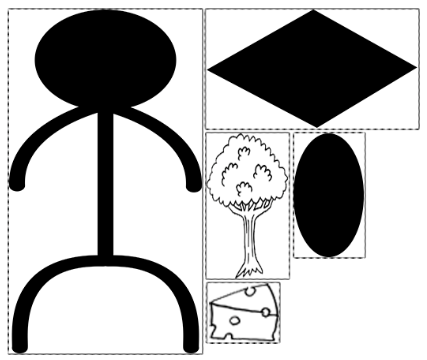
\includegraphics[scale=0.7]{img/boundingBox.png}
\caption{Illustration du procédé des bounding boxes}
\label{fig:boundingBox}
\end{figure}

\indent Les deux premiers solveurs, \texttt{LineSolver} et \texttt{MultilineSolver} sont des plus basiques, mais ils permettent au moins de disposer les pièces sur les plaques sans intersection. L'algorithme \texttt{ScanLineSolver} est plus complexe et fournit une bien meilleure compacité.\\

L'algorithme \texttt{LineSolver} se contente d'aligner les formes de façon désordonnée sur une ligne, sans retour lorsque l'on dépasse la taille de la plaque. Pour cela il colle les rectangles entre eux au plus proche. Lorsque la largeur de la plaque est dépassée, il passe à une plaque suivante.\\

L'algorithme \texttt{MultilineSolver} en est une version améliorée. Les différentes boîtes sont triées par hauteur et sont placées par hauteurs décroissantes.
Le packing va alors se faire ligne par ligne, en insérant les pièces depuis le bord gauche jusqu'à atteindre le bord droit de la plaque. Les lignes sont ensuite juxtaposées les unes en dessous des autres. Un exemple de sortie peut être constaté en figure~\ref{fig:multilineSolver}.

\begin{figure}[!htb]
\centering
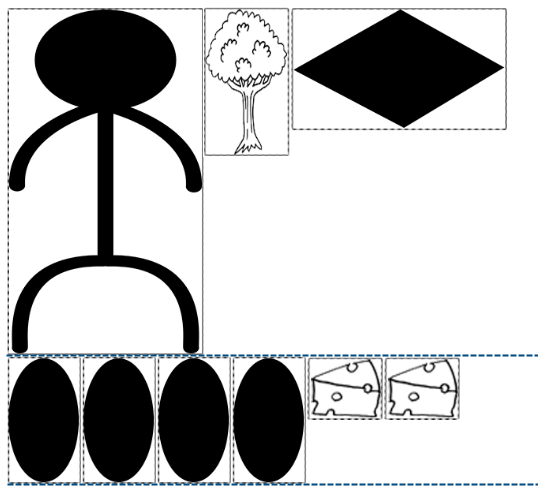
\includegraphics[scale=0.6]{img/multilineSolver.png}
\caption{Exemple d'une sortie du \texttt{MultilineSolver}}
\label{fig:multilineSolver}
\end{figure}

Le solveur \texttt{ScanLine} utilise l'algorithme connu du \textit{first-fit}. Il commence par affiner la boîte englobante au mieux : des rotations sont effectuées sur les pièces afin d'obtenir la boîte avec un rapport (aire vide / aire boîte) le plus faible. Ces boîtes sont ensuite triées par ordre décroissant de hauteur, comme l'illustrent la figure~\ref{fig:ScanlineA}.

\begin{figure}[!htb]
\centering
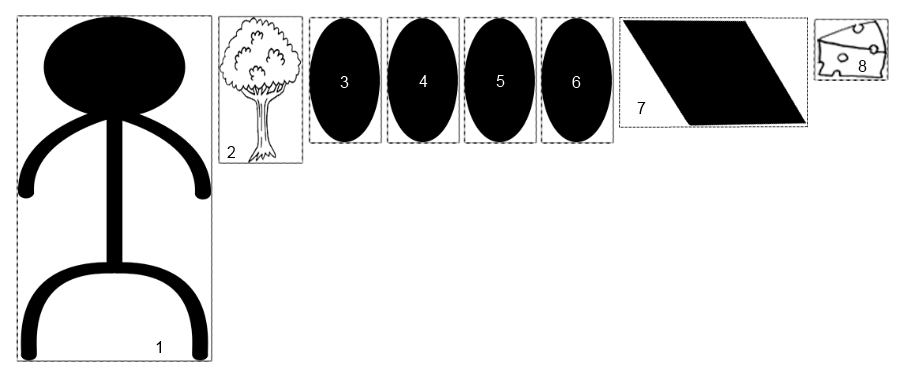
\includegraphics[scale=0.6]{img/ScanlineA.png}
\caption{Jeu de pièces, affinées à la meilleure bounding box, puis triées}
\label{fig:ScanlineA}
\end{figure}

\newpage
\indent L'essentiel du packing va consister à manipuler une grille de cellules rectangulaires dans l'état "plein" ou "vide", et de déterminer un ensemble de cellules dans lequel une boîte peut rentrer. Le parcours de cette grille s'effectue colonne par colonne de haut en bas, de gauche à droite. Dès qu'une place est trouvée pour la boîte, c'est-à-dire un ensemble de cellules toutes vides, la grille est mise à jour pour correspondre exactement aux nouvelles cellules pleines et vides avec les boîtes placées (figure~\ref{fig:ScanlineC2-3}).

\begin{figure}[!htb]
\centering
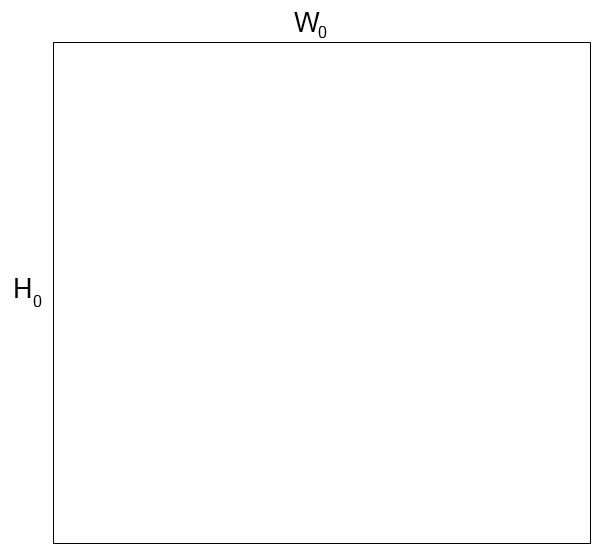
\includegraphics[scale=0.4]{img/ScanlineC1.png}
\caption{La plaque initiale est une grille à une seule cellule vide}
\label{fig:ScanlineC1}
\end{figure}

\begin{figure*}[!htb]
    \centering
    \begin{subfigure}{.48\linewidth}
        \centering
        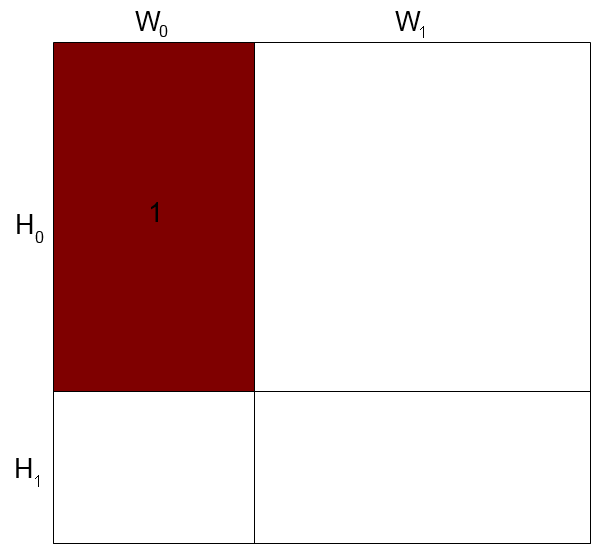
\includegraphics[width=\linewidth]{img/ScanlineC2.png}
        \caption{Ajout de la pièce 1 en $(W_0,H_0)$}
    \end{subfigure}%
    ~ 
    \begin{subfigure}{.48\linewidth}
        \centering
        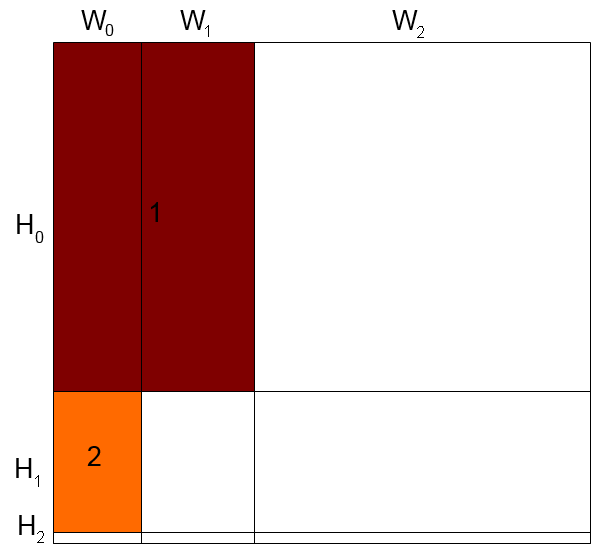
\includegraphics[width=\linewidth]{img/ScanlineC3.png}
        \caption{Ajout de la pièce 2 en $(W_0,H_1)$}
    \end{subfigure}
    \caption{A chaque ajout de pièce, la grille est redécoupée}
    \label{fig:ScanlineC2-3}
\end{figure*}

\begin{figure*}[!htb]
    \centering
    \begin{subfigure}{.48\linewidth}
        \centering
        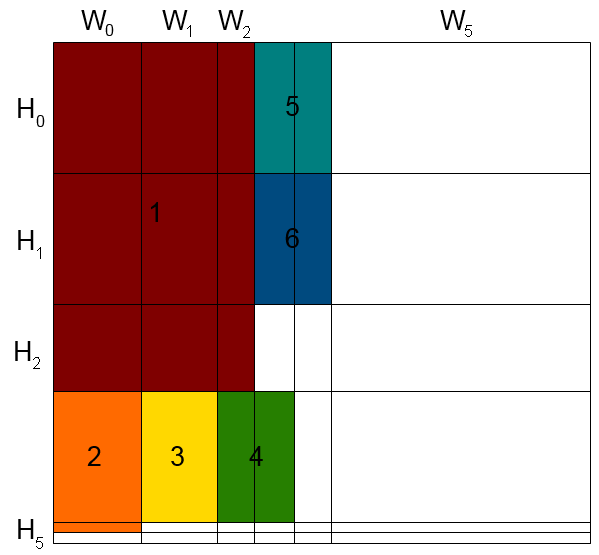
\includegraphics[width=\linewidth]{img/ScanlineC4.png}
        \caption{Grille après insertions des pièces 1 à 6}
    \end{subfigure}%
    ~ 
    \begin{subfigure}{.48\linewidth}
        \centering
        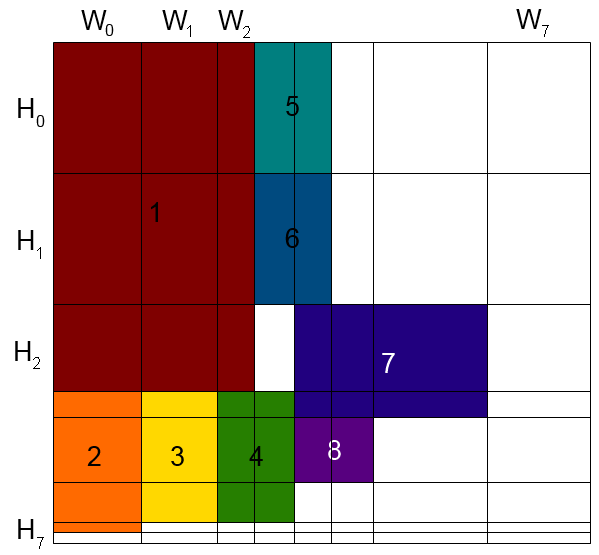
\includegraphics[width=\linewidth]{img/ScanlineC5.png}
        \caption{Les insertions peuvent créer des trous}
    \end{subfigure}
    \caption{Une pièce s'insère le plus à gauche, puis le plus en haut possible}
    \label{fig:ScanlineC4-5}
\end{figure*}

\begin{figure}[!htb]
\centering
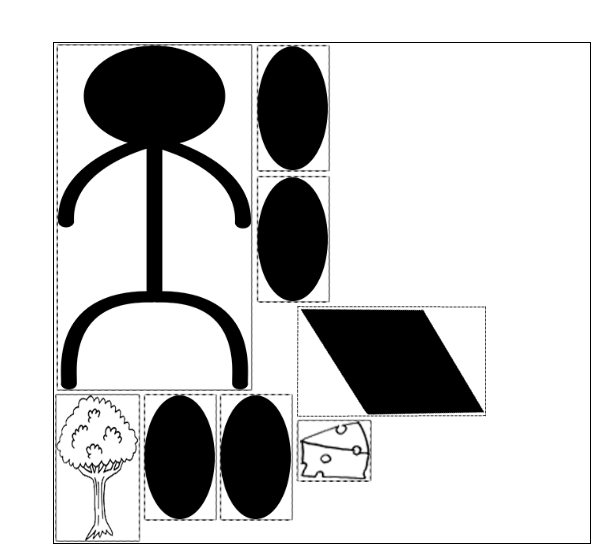
\includegraphics[scale=0.5]{img/ScanlineC6.png}
\caption{Sortie de l'algorithme \texttt{ScanlineSolver}}
\label{fig:ScanlineC6}
\end{figure}

\newpage
\indent Il se peut que la succession des insertions et la maximisation de la compacité laisse une cellule vide entre les pièces, les plus grandes ne pouvant pas s'y placer (figure~\ref{fig:ScanlineC4-5}). Toutefois les pièces sont triées par ordre décroissant de hauteur, aussi les pièces les plus petites combleront ces cellules vides pour améliorer davantage la compacité de la plaque finale.

\newpage
Enfin, une dernière optimisation est effectuée une fois que toutes les pièces ont tenté une insertion: ces pièces sont tournées de 90°, puis un nouvel essai est effectué quant à leur insertion. Cela conserve les propriétés rectangulaires dont le solver a besoin, et une pièce plus large que longue peut donc rentrer dans un ensemble de cellules jusque-là trop petit.

\begin{figure}[!htb]
\centering

\includegraphics[scale=0.5]{img/ScanlineClounk.png}
\caption{Une pièce trop large peut être insérée après rotation}
\label{fig:ScanlineClounk}
\end{figure}


\subsubsection{Algorithmes non déterministes}

Les autres algorithmes implémentés insèrent les pièces de manière partiellement aléatoire sur la plaque.\\

Le solver \texttt{FreezeSolver} assimile la plaque à un panier que l'on remplit, et fait tomber les pièces une à une dans la plaque grâce à de petites translations qui simulent la gravité pendant un certain nombre d'itérations.\\
\indent La pièce tombe alors vers le bas de la plaque et en cas de collision avec les bords ou le fond, la pièce est repoussée vers l'intérieur. Après un certain temps de calcul, le solver vérifie que la position de la pièce est valide (c'est-à-dire entièrement dans la plaque, et sans collision générée par les dernières translations-rotations), la pièce se fige et la suivante est lâchée à partir du haut (figure~\ref{fig:FreezeAB}).\\

\begin{figure*}[!htb]
    \centering
    \begin{subfigure}{.4\linewidth}
        \centering
        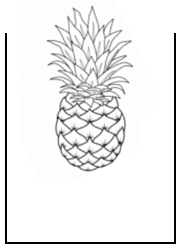
\includegraphics[width=\linewidth]{img/FreezeA.png}
        \caption{La pièce 1 est lachée du haut de la plaque}
    \end{subfigure}%
    ~ 
    \begin{subfigure}{.4\linewidth}
        \centering
        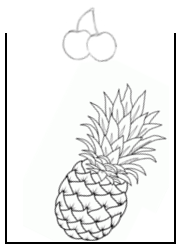
\includegraphics[width=\linewidth]{img/FreezeB.png}
        \caption{La pièce 1 se fige, et la pièce 2 est lachée}
    \end{subfigure}
    \caption{Le \texttt{FreezeSolver} s'apparente à un panier}
    \label{fig:FreezeAB}
\end{figure*}


\indent Si une pièce entre entre collision avec une autre lors du calcul, alors elle est expulsée vers le haut, translatée aléatoirement à gauche ou à droite, et pivotée aléatoirement dans un sens ou dans l'autre avant de recommencer à tomber, ce qui simule un entassement des pièces dans la plaque (figure~\ref{fig:FreezeCD}).\\

\begin{figure*}[!htb]
    \centering
    \begin{subfigure}{.30\linewidth}
        \centering
        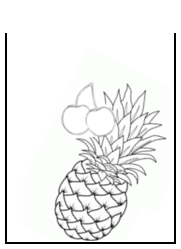
\includegraphics[width=\linewidth]{img/FreezeC.png}
    \end{subfigure}%
    ~ 
    \begin{subfigure}{.30\linewidth}
        \centering
        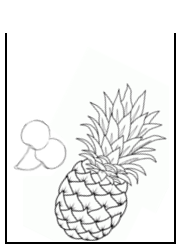
\includegraphics[width=\linewidth]{img/FreezeD.png}
    \end{subfigure}
    ~ 
    \begin{subfigure}{.30\linewidth}
        \centering
        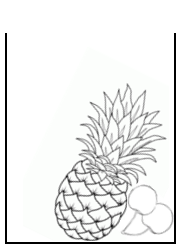
\includegraphics[width=\linewidth]{img/FreezeE.png}
    \end{subfigure}
    
    \caption{Lors d'une collision, la pièce est repoussée à gauche ou à droite}
    \label{fig:FreezeCD}
\end{figure*}

\newpage
\indent De plus, si le solver n'arrive pas à stabiliser la pièce, c'est-à-dire si elle est toujours en collision avec une autre après de multiples essais de corrections, celle-ci est envoyée vers une seconde plaque pour être packée. Cela se produit naturellement lorsque la plaque est déjà saturée et ''déborde''.

\begin{figure}[!htb]
\centering
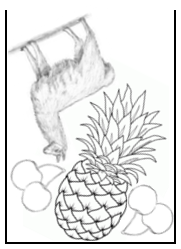
\includegraphics[scale=1]{img/FreezeG.png}
\caption{Sortie de l'algorithme \texttt{FreezeSolver}}
\label{fig:FreezeSolver}
\end{figure}




\newpage

PROBASOLVER

\begin{figure}[!htb]
\centering

\includegraphics[scale=2]{img/Trombi.jpg}
\caption{Bonjour. Il semble que cette partie n'a pas encore été écrite.}
\end{figure}

\newpage




% Quelques chiffres:

% Multiline :
% Scanline :
% Freeze :
% Proba :